\documentclass[11pt,a4paper,twoside,openright]{article}
\usepackage[utf8]{inputenc}
\usepackage[english]{babel} % define document language
% \usepackage{datetime}  
\usepackage[T1]{fontenc}
\usepackage{arydshln}
\usepackage{enumitem}
\usepackage{wrapfig}
\usepackage{bbold} % fct indicatrice

\usepackage{tikz}


\usepackage{url}
\usepackage[colorlinks,linkcolor=red,anchorcolor=green,citecolor=blue]{hyperref}

\usepackage{lmodern}
% \usepackage[hidelinks]{hyperref} % Hyperref package for url's and [hidelinks] option to remove collouring


\linespread{1.2}

\usepackage{amsmath,amsthm,amssymb,amsfonts}
\DeclareMathOperator*{\argmax}{arg\,max}
\DeclareMathOperator*{\argmin}{arg\,min}
\usepackage{graphicx} 
\usepackage{float} 
\usepackage{subfigure}
\usepackage{caption}
% \renewcommand{\thesubfigure}{(\roman{subfigure})}


% section title size
\usepackage{titlesec}
\titleformat*{\section}{\huge\bfseries}
\titleformat*{\subsection}{\Large\bfseries}
\titleformat*{\subsubsection}{\large\bfseries}


% \graphicspath{ {./images/} }

%marges
\usepackage{geometry}
\geometry{top= 3 cm, bottom= 3 cm, right= 2.5 cm, left= 3 cm, headheight=13.6pt}

% extra section for paragraph
\usepackage{titlesec}
\setcounter{secnumdepth}{4}
\setcounter{tocdepth}{4}
\titleformat{\paragraph}
{\normalfont\normalsize\bfseries}{\theparagraph}{1em}{}
\titlespacing*{\paragraph}
{0pt}{3.25ex plus 1ex minus .2ex}{1.5ex plus .2ex}


% % % extra section for subparagraph
% % \usepackage{titlesec}
% \setcounter{secnumdepth}{5}
% \setcounter{tocdepth}{5}
% \titleformat{\subparagraph}
% {\normalfont\normalsize\bfseries}{\thesubparagraph}{1em}{}
% \titlespacing*{\subparagraph}
% {0pt}{3.25ex plus 1ex minus .2ex}{1.5ex plus .2ex}


% % codes
% \usepackage{minted}

\newtheorem{exemple}{Exemple}

% abstract
\renewenvironment{abstract}
 {\quotation\small\noindent\rule{\linewidth}{.5pt}\par\smallskip
  {\centering\bfseries\abstractname\par}\medskip}
 {\par\noindent\rule{\linewidth}{.5pt}\endquotation}



% biblio 
\usepackage[
backend=biber,
style=alphabetic,
sorting=nyt
]{biblatex}
\usepackage{csquotes}



\usepackage[toc]{glossaries}

% \makeglossaries
\makenoidxglossaries


\newglossaryentry{put}
{
    name= {put}, % reference name for this glossary term
    description={A put option in finance is\dots)}
}



\newglossaryentry{call}
{
    name= {call},
    description={call option is ...}
}


% \renewcommand{\glstextformat}[1]{\color{black}  #1}
\renewcommand{\glstextformat}[1]{\color{blue}  #1}

\addbibresource{bibfile.bib}

\usepackage[utf8]{inputenc}
\usepackage{mathrsfs}
\newtheorem{thm}{Théorème}
\newtheorem*{thm*}{Théorème}

\usepackage[figurename=Fig.]{caption}
\usepackage[tablename=Tab.]{caption}

\newcommand\watermark{Non terminé}
\usepackage[color={[RGB]{255,191,191}}, text=\watermark, scale=1]{draftwatermark}

\usepackage{fancyhdr,graphicx,lastpage}
\fancypagestyle{plain}{
  \fancyhf{}
  \fancyhead[R]{\textit{Rapport d'activités en entreprise}}% tête de page droit
  \fancyhead[L]{\textit{Alexis Déhu}}% tête de page à gauche
  \fancyfoot[L]{\textit{2023-2024}}% pied de page à gauche
  \fancyfoot[R]{\thepage\  / \pageref{LastPage}}% pied de page à droite
}
\pagestyle{plain}

\begin{document}
\begin{sloppypar}
\pagestyle{empty}

% Declare new goemetry for the title page only.
\newgeometry{margin=1in}

% variables
\newcommand\titreDocument{\bfseries Rapport d'activités}
\newcommand\poste{Apprenti Administrateur Systèmes et Réseaux en alternance}
\newcommand\auteurDocument{Alexis Déhu}
\newcommand\dateRendu{\bfseries le 31 Mai 2024}
\newcommand\nomResponsable{M. Éric Pierre-Sala}
\newcommand\nomTuteur{M. Guillaume Devesa}
\newcommand\nomEnseignantReferant{M. Angel Abénia}
\newcommand\nomFormation{BUT Réseaux et Télécommunications parcours Cybersécurité, 2ème année}
\newcommand\nomEntreprise{ADITU, Technopole Izarbel Côte Basque, 64210 Bidart}

\begin{titlepage}
   \begin{center}

        % détachement du haut de la page
        \vspace*{2cm}

        % logo de l'université, de l'établissement et du département
        \href{https://www.univ-pau.fr/}{
\includegraphics[width=0.25\textwidth]{images/logo/uppa.png}}
        \quad \quad
        \href{https://iutpa.univ-pau.fr/fr/index.html}{
\includegraphics[width=0.25\textwidth]{images/logo/iut.jpg}}
        \quad
        \href{https://iutpa.univ-pau.fr/fr/l-iut/nos-campus/campus-de-mont-de-marsan.html}{
\includegraphics[width=0.25\textwidth]{images/logo/mdm.png}}\\

        % bande horizontale
        \noindent\rule[0.25\baselineskip]{\textwidth}{1pt}

        % espacement de la bare horizontale avec le titre du document
        \vspace{0.5 cm} 

        \Huge{\titreDocument} 

        \vspace{0.5cm}
        \LARGE{\poste}
          
        \vspace{2.5 cm}
        \large{\auteurDocument}\\
        \large{\dateRendu}\\

        \vspace{4 cm}
         
        \leftline{\small{\textbf{Responsable :} \nomResponsable}}
        \leftline{\small{\textbf{Maître d'apprentissage :} \nomTuteur}}
        \leftline{\small{\textbf{Enseignant référent :} \nomEnseignantReferant}}

        \vspace{1 cm}

        \leftline{\small{\textbf{Formation :} \nomFormation}}
        \leftline{\small{\textbf{Entreprise d'accueil :} \nomEntreprise}}

        % retour de la barre horizontale
        \noindent\rule[0.25\baselineskip]{\textwidth}{1pt}\\
        
        \href{https://www.aditu.fr/}{
\includegraphics[width=0.25\textwidth]{images/logo/aditu.png}}
        \quad \quad
        \href{https://www.datacube-services.fr/}{
\includegraphics[width=0.11\textwidth]{images/logo/data3.png}}\\
      
    \end{center}
\setcounter{page}{0}
\end{titlepage}

\restoregeometry

\newpage

\thispagestyle{empty}
\mbox{}

\newpage

\centerline{\huge{\textbf{Remerciements}}}

\vspace{1 cm}

\textit{à faire}

\newpage
\renewcommand*\contentsname{Table des matières}
\tableofcontents

\newpage
\setcounter{page}{1}
\pagestyle{plain}
\section{Introduction}

Le présent document est le compte rendu de mes activités au sein de l’entreprise ADITU pour les périodes d’alternance du 1er Septembre 2023 au 31 Mai 2024 (39 semaines effectives pour 26 en entreprise) en tant qu’Apprenti Administrateur Systèmes et Réseaux.
\\ \\
Cet apprentissage en alternance a été réalisé dans le cadre de l’obtention d’un BUT en Réseaux \& Télécommunications à l’Université de Pau et des Pays de l’Adour, IUT de Mont-de-Marsan. La période d’alternance d’une durée de 2 ans s’est établie du 1er Septembre 2023 au 31 Août 2025 dans les locaux d’ADITU, Technopole Izarbel Côte Basque, 64210 Bidart.
\\ \\
L'apprentissage se déroulait par le biai de projets répondant à des problèmatiques abordant des infrastructures croissement critiques dans l'activité de l'entreprise. Ainsi, je me suis successivement vu attribuer les projets d'instaurer des applications en internes pour faciliter le travail de l'équipe, réorganiser le système de connexion à distance aux machines, créer une centrale d'observation de l'accessibilité des sites WEB, solutionner une nouvelle application de support client et procédurer l'assainissement et la mise à jour d'équipements utilisés en production. De plus grands projets d'une criticité plus importante sont encore en cours de complétion.
\\ \\
Sera présentée l'entreprise en revenant sur la raison de sa création et comment celle-ci y répond encore aujourd'hui, en abordant ses équipes, son organisation et les services proposés pour sa clientèle définie. Sera ensuite couvert mes activités au cours de cette année d'apprentissage, en revenant sur les besoins clairs de mes projets, ce que j'y ai apporté et appris; pour terminer sur un bilan horaire et sur leurs résultats. J'en suivrai par une conclusion sur ce que ces activités m'ont apportés professionnellement avec quelques perspectives de réflexion, pour en finir avec un bilan personnel sur cette première année d'expérience.
\\ \\
Aucune intelligence artificielle n’a été utilisée pour la rédaction ou l’aide à la production de ce document. Aucune information présente n’a été récupérée brute de forme depuis quelconque source, publique ou non. Ce document est le fruit d’un travail personnel et que je n’ai ni contrefait, ni falsifié, ni copié tout ou partie de l’œuvre d’autrui afin de la faire passer pour mienne.
% \\ \\
% Rapport d’activités en entreprise ADITU 12/02/2024-08/03/2024 © 2024 by Alexis Déhu is licensed under CC BY-NC-ND 4.0

\newpage

\section{Présentation de l'entreprise d'accueil}
ADITU fut fondée en 2004 en tant que première Délégation de Service Public en France dans le domaine des services aux entreprises. Sa création fut initiée par la Communauté d’Agglomération Côte Basque-Adour (Bayonne, Anglet, Biarritz, Boucau et Bidart).
\\ \\
Son implémentation se fut à la Technopole Izarbel à Bidart avec pour objectif de permettre aux entreprises du secteur de se reposer sur les services informatiques d'ADITU pour se reconcentrer sur leurs activités professionnelles.
\\ \\
Son équipe est constituée essentiellement de personnels techniques, à savoir des techniciens et administrateurs de systèmes et de réseaux informatiques. Pour nous guider sont présents M. Guillaume Devesa notre Directeur technique et M. Éric Pierre-Sala le Directeur, épaulée par Mme. Marina Galant pour la partie commerciale, communication et administrative.
\begin{figure}[H] % H fixed h flexible
  \centering
  \captionsetup{justification=centering}
  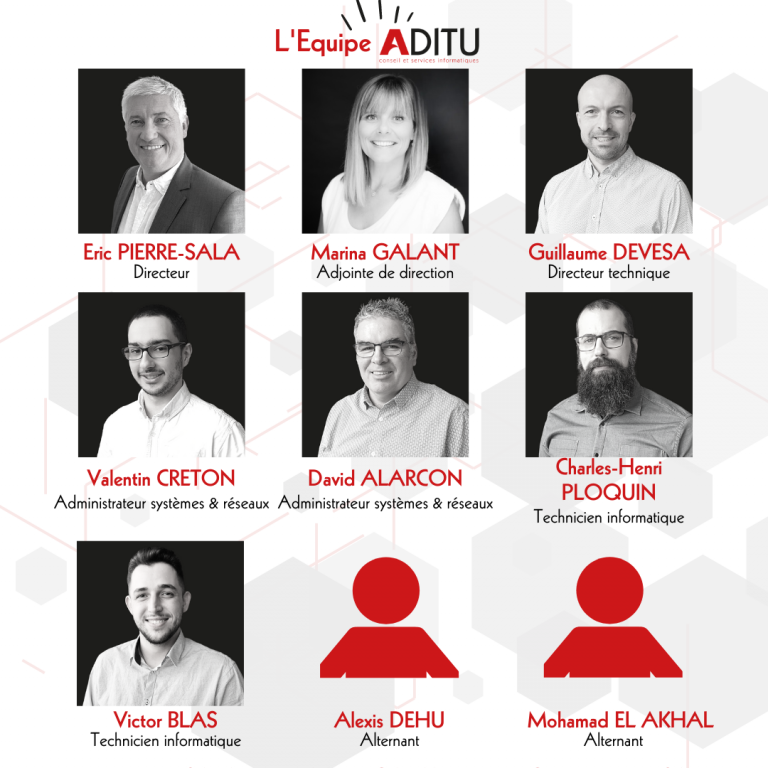
\includegraphics[scale = 0.5]{images/equipe_aditu.png}
  \caption{Membres de l'équipe d'ADITU lors mon alternance.}  
  \label{fig:aditu_members} % pour la citer après
\end{figure}

\subsection{Secteur d'activité professionnel}

Le secteur d'activité d'ADITU se caractérise par la réponse aux besoins d'aider les entreprises du secteur à se développer rapidement et efficacement en les déchargeant de l'élaboration ou le maintient de leur infrastructure informatique. ADITU tend à être l'intermédiaire des professionnels locaux au monde du numérique.
\\ \\
ADITU permet à ses clients de pouvoir se concentrer sur leur activité professionnelle en les déchargeant de l'utilisation d'une infrastructure faillible, vieillissante ou incorrectement maintenue (perte de données, complexité d'utilisation, problème d'expansibilité, failles de sécurités...).  
\\ \\
Le secteur d'activité est solide, assurant aux entreprises leur bon fonctionnement sans qu'elles aient besoin de former ou d'embaucher une personne technique pour maintenir leurs infrastructures. L'équipe d'ADITU travail à la performance et à la refocalisation des entreprises sur leurs activités professionnelles.

\subsection{Clientèle ciblée et son étude}

ADITU a été fondé en soutient aux entreprises du Pays Basque, des Landes et du Béarn. Sa zone d'attractivité s'étend dans ces régions. Cette zone de chalandise reste locale mais très éclatée sur la côte Basque. Le Directeur M. Éric Pierre-Sala souhaite que l'entreprise garde cette proximité avec ses clients et ses acteurs, pour conserver une relation humaine force d'ADITU.
\\ \\
La clientèle ciblée est variée, regroupant entreprises et organisations locales ayant besoin d'externaliser tout ou partie de la gestion de leur infrastructure numérique. La plupart des clients d'ADITU sont des clients "historiques" de toute taille avec au moins de dix années d'ancienneté.
\\ \\
Les clients d'ADITU sont des clients souhaitant de la proximité et de l'humain pour leur informatique, pouvant communiquer rapidement avec une personne. Ces personnes sont souvent rattachés à leur région de par leur activité économique ou commerciale, et sont demandeurs d'acteurs locaux.
\\ \\
La différence de taille parmi les clients reste variée : pouvant aller d'un grand groupe souhaitant s'installer dans le Pays Basque à une PME dans le besoin de quelques services.

\subsection{Services distribués à sa clientèle}

Pour répondre aux besoins du secteur, ADITU propose des services de conseils, d'installation et de maintenance d'infrastructures informatiques à la demande pour ses clients. Chaque client peut choisir la souscription d'un ou plusieurs services selon leurs besoins et le support souhaité.
\\ \\
Pour assurer la continuité des services proposés, ADITU possède deux data centres \textit{(Centres d'hébergement et de Gestion des données)}, à Bidart et à Dax. Ces data centres servent à \textbf{l'hébergement} de machines dédiées aux clients ou à l'hébergement de leurs services que nous maintenons continuellement (sites WEB, messagerie, stockage et partage de fichiers, systèmes de sauvegardes, applications métier...).
\\ \\
ADITU propose aussi la supervision du fonctionnement des services de ses clients hébergés en data centres ou sur leurs sites. Le service \textbf{d'infogérance} permet aux clients d'être informés en tant réel de la disponibilité de leurs services pour leurs collaborateurs, et d'être rassurés de la remise en fonctionnement et du suivi de ces services. L'infogérance englobe le support téléphonique et informatique, et l'aide à la résolution de problèmes quotidien.
\\ \\
Des journées en \textbf{régie} sont proposées, permettant l'envoi d'un technicien dédié au support et au contrôle du bon fonctionnement de l'infrastructure sur l'ensemble d'une journée. Le technicien est alors sollicité pour des problèmes mineurs, des formations, de l'installation de matériel etc. Ce type de journées est intéressant pour la vérification d'une utilisation propre de l'infrastructure installée et pour faciliter l'activité du client.

\subsection{Organisation des équipes}

Niveau organisationnel, l'équipe technique se réunit chaque lundi matin avec le dirigeant pour planifier les actions de la semaine suivant les retours et les appels des clients, des journées en régie ou autres retours obtenus. Cette réunion est dite d'exploitation.
\\ \\
Cette réunion est suivie d'un point technique commun à toute l'équipe technique où sont discutés les progrès de la semaine précédente avec les potentiels points bloquants, puis de la méthodologie d'approche du travail de la semaine défini dans la réunion d'exploitation. Le tout sous conseil et la supervision d'ensemble de l'équipe.
\\ \\
Plusieurs réunions, points ou comités peuvent être organisés dans la semaine, planifiés lors de la réunion d'exploitation de la semaine ou plusieurs semaines à l'avance.
\\ \\
Chaque jour, une personne est aussi dite "de support", travaillant sur ses projets et répondant aux demandes de support des clients. Cela permet à tous les membres de l'équipe de pouvoir se consacrer à ses projets sans devoir penser à répondre constamment aux appels.

\newpage

\section{Activités en entreprise}

Mes journées dans l'entreprise étaient rythmées par le fil directeur des projets que je me visualisais. J'avais une vision d'ensemble de l'objet final qui m'était donné par mon maître d'apprentissage par un cahier des charges, et je m'organisais au mieux pour documenter et fournir un travail propre du début à sa fin.
\\ \\
Plusieurs projets m'ont alors été confiés, pour la plupart terminés mais pour ceux les plus récents encore en cours de concrétisation.

\subsection{Projets accomplis}

Les projets terminés sont ceux obtenus à mon entrée dans l'entreprise, ceux de moyenne ou de petite taille, ou ceux pour lesquels j'avais une partie des connaissances nécessaires pour les aborder avant de les étudier. J'ai ainsi procédé à différentes activités dans l'entreprise chronologiquement dans l'ordre suivant.

\subsubsection{Montage de services d'administration et de partage}

Définie dans la fiche de poste à mon arrivée dans l'entreprise, était demandée une collection d'applicatifs répondant à des besoins de l'équipe pour faciliter leur travail quotidien. Ceux-ci n'étaient pas présents auparavant par manque de temps pour les mettre en place, les maintenir ainsi que pour monter en compétences dans certains domaines touchés.
\\ \\
Voici la liste des solutions que j'ai déployées la première période, en écoute des besoins de mes collègues et de ma fiche de poste pour faciliter le travail quotidien de l'équipe en interne et envers les clients.

\begin{itemize}
  \item Une \textbf{interface de gestion d'applications conteneurisées}
  \item Un \textbf{serveur mandataire d'accès inverse}.
  \item Une \textbf{solution de partage de mots de passe sécurisée}.
  \item Une \textbf{plateforme d'échange de fichiers volumineux}.
  \item Une \textbf{console de vérification de disponibilité des sites hébergés}.
  \item Une \textbf{infrastructure de développement et d'échange de code}.
\end{itemize}

\noindent Tout mon travail fut de comprendre les intérêts de l'équipe pour approcher ces solutions en répondant au mieux à leur besoin initial, et dans le pire des cas y trouver une alternative; mais aussi de mettre au point ses solutions, de manière sécurisée et stable.

\paragraph{L'intérêt de l'interfaçage pour une application en équipe}

Les solutions fonctionnent sous forme de micro-services, dit "conteneurisés", en utilisant la technologie Docker. Celle-ci permet de réduire l'empreinte des solutions lancées et de facilement pouvoir les maintenir.% : les redémarrer, les mettre à jour et les réagencer stablement.
% Docker permet un contrôle de version des applicatifs pour facilement revenir sur une ancienne version si les mises à jour sont conflictuelles, une intégration simple avec les autres micro-services, une facilité dans leur déploiement et j'en passe.
\\ \\
L'inconvénient de cette technologie est qu'elle a besoin d'être appréhendée en formations pour s'en servir correctement car complexe à l'accommodation - possible uniquement en lignes de commande. C'est pour cela que toujours pour aider l'équipe au quotidien j'ai implémenté une interface pour gérer ces micro-services par le suivis d'actions plutôt que par des commandes.
\\ \\
L'équipe peut désormais profiter de la flexibilité et des fonctionnalités de Docker en utilisant une interface et en lisant des procédures plutôt que d'apprendre et devoir prendre en main la technologie.
\\ \\
J'ai appris en entreprise que l'on ne travaille pas pour soit ni seul, mais généralement en équipe et ici pour une équipe. Je pouvais monter les meilleurs services selon moi, mais ceux-ci n'auraient peut-être pas été accessibles pour tout le monde n'ayant pas le même raisonnement ou connaissances devant la solution.
\\ \\
J'en retiens ici de favoriser l'accessibilité aux fonctionnalités lorsque cela est nécessaire, sur le moment et plus tard lorsqu'une personne devra reprendre le projet (comme ce fut le cas pour moi); en documentant mon travail, en y ajoutant des procédures détaillées et en essayant de conserver le nécessaire au meilleur si cela complexifie trop le travail.
\\ \\
Au fur et à mesure que je travaillais avec les technologies de l'entreprise et Docker, je me suis plus à en apprendre davantage sur elles.

\paragraph{Le rôle d'un serveur mandataire d'accès inverse en entreprise}

A été monté un serveur mandataire d'accès inverse, aussi dit Reverse Proxy, pour hébergés les micro-services.
\\ \\
Un serveur mandataire d'accès est un serveur par lequel les utilisateurs sont obligés de demander (mandataire) pour accéder à un ou plusieurs services (serveur d'accès), généralement sur Internet.
\\ \\
Ainsi, dans les universités ou autres institutions sont souvent installés de manière transparente un serveur mandataire d'accès pour limiter l'activité des utilisateurs sur Internet car bloqué par le serveur d'accès, ou pour journaliser leurs activités.
\\ \\
Un serveur mandataire d'accès inverse effectue les mêmes opérations dans le sens inverse : il laisse les utilisateurs accéder à des ressources, mais journalise leurs activités et permet l'utilisation de services en passant par un passage unique d'entrée exposé à l'extérieur.
\\ \\
Son intérêt devient crucial en sécurité, amincissant la surface d'attaque possible des sites d'une entreprise en faisant circuler les connexions par un seul endroit journalisant les informations.

\begin{figure}[H] % H fixed h flexible
  \centering
  \captionsetup{justification=centering}
  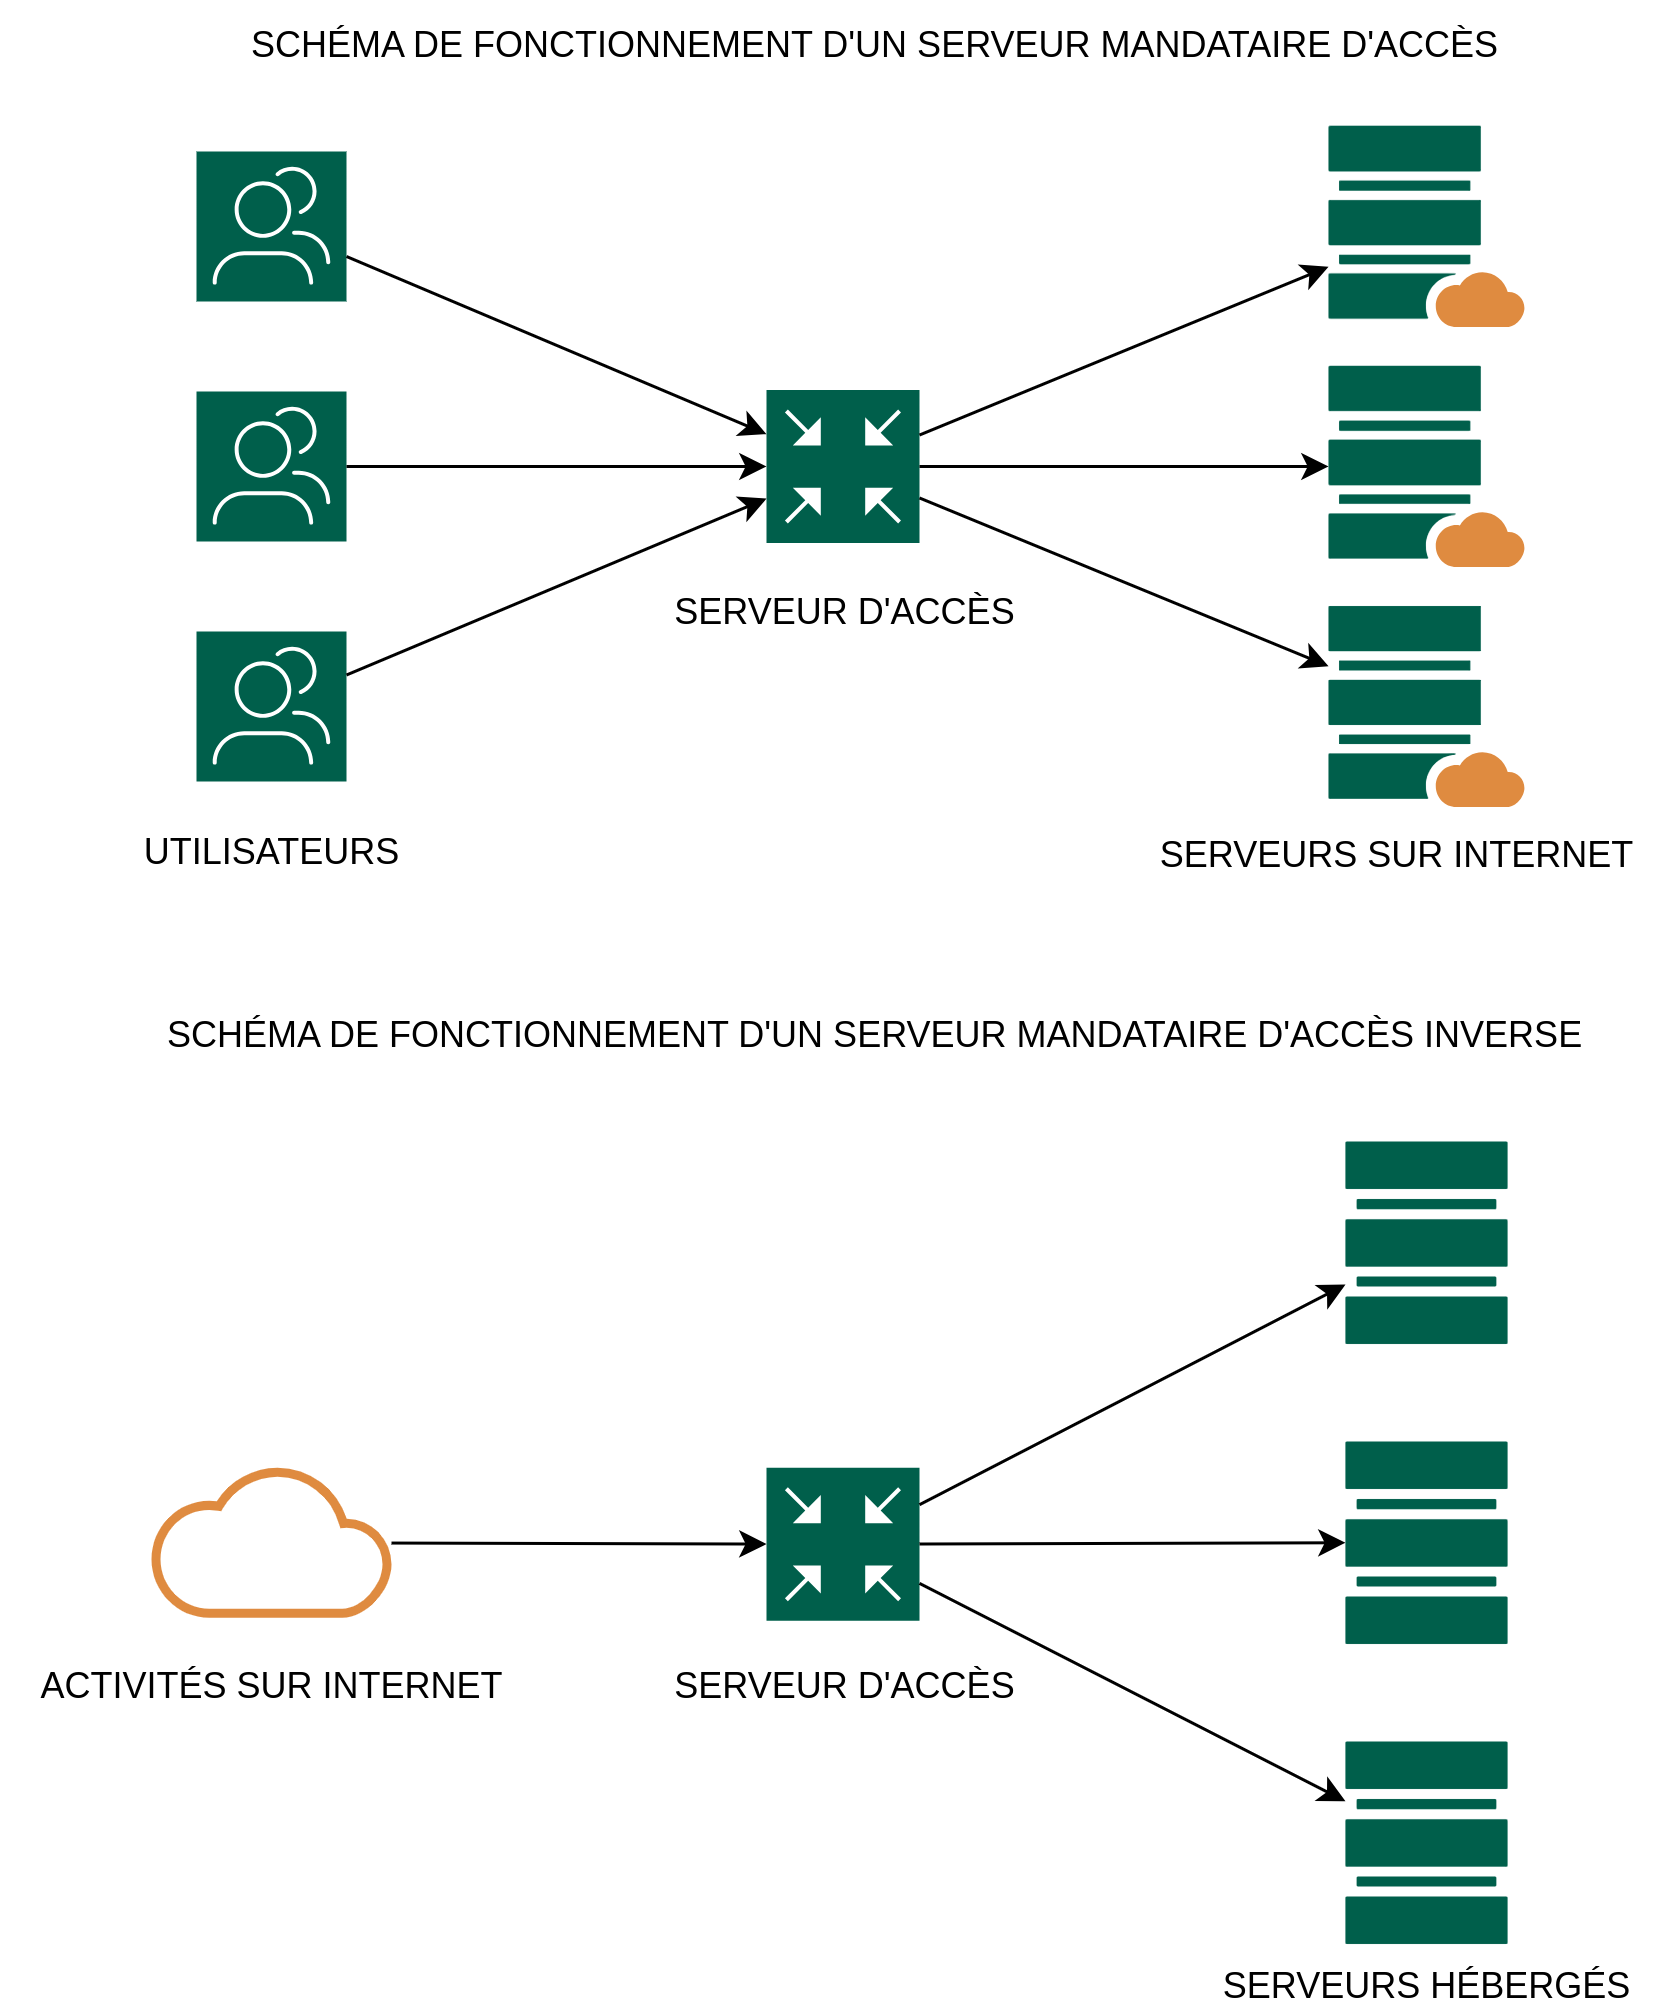
\includegraphics[scale = 0.2]{images/serveur_mandataire_acces.png}
  \caption{Schéma de fonctionnement d'un serveur mandataire d'accès et d'un serveur mandataire d'accès inverse.}  
  \label{fig:serveur_mandataire_acces} % pour la citer après
\end{figure}

\noindent J'ai ainsi monté un serveur mandataire d'accès inverse pour toutes les solutions hébergées, lui-même étant un micro-service sous Docker. En résultant une exposition contrôlée des solutions hébergées et accessibles depuis l'extérieur, notamment par nos clients.

\paragraph{Découverte de l'importance d'échanger les mots de passe de manière chiffrée avec les clients}

Lors de mon arrivée dans l'entreprise, j'ai remarqué qu'il n'y avait pas de politique d'échange de mots de passe avec les clients. Certaines personnes de l'équipe envoyaient les mots de passe en texte par courriel, d'autres par des liens de services dédiés pour faire accéder aux clients leurs mots de passe sans le divulguer explicitement dans les courriels.
\\ \\
Je me suis aussi rendu compte que, parce que non initiés aux bonnes pratiques, nos clients utilisent souvent des mots de passe faillibles. 
% gens pas habilent utilisent mots de passes faibles
% qui en plus sont envoyés en clair par mail
\\ \\
\underline{\textbf{PAS CONTINUE NI FAIT LES 3 AUTRES, CAR JE NE SAIS PAS SI C'EST UTILE}}
\\
\underline{\textbf{OU HORS-SUJET DE CONTINUER DANS CETTE VOIE}}

\subsubsection{Étude et mise en production d'une nouvelle solution de support en ligne}

ADITU possède trois moyens de communication avec ses clients : les courriels, les échanges téléphoniques et une solution de support par ouverture de tickets. Par la dernière, les clients ouvrent un ticket pour une demande ou un problème qu'ils rencontrent et s'assurent d'un suivi clair et pérenne de leur démarche à ce seul endroit (pas le cas pour les courriels ou par téléphone).
\\ \\
Cette dernière était cependant la moins utilisée, nos clients la trouvant vieillissante des trois solutions de support, simpliste et non agréable visuellement et à l’utilisation. De notre côté, l'équipe se plaignait également du manque de praticité pour la gestion des tickets et d’une trop faible flexibilité dans son utilisation (impossible de faire du cas par cas).
\\ \\
Mon travail fut de rechercher une nouvelle solution professionnelle de support en élaborant une étude comparative des solutions sur le marché, de les étudier comportementalement en environnement contrôlé pour m'assurer qu'elles répondaient bien aux besoins dans leur pratique; pour terminer sur la mise en production de la solution conservée et la vérification de sa bonne utilisation et de compréhension par les clients.
\\ \\
Un de mes projets fil rouge chez ADITU, l'étude comparative et les mises en situation furent longues et intéressantes. J'y ai notamment appris que lors d'une étude comparative, il fallait comparer les solutions sur les besoins qu'elles devaient répondre plutôt que sur les fonctionnalités que chacune proposait.
\\ \\
En effet, nous voulions pas choisir la meilleure solution mais celle qui répondait au mieux à nos besoins. Ainsi, j'ai pris l'initiative de noter les solution de 0 à 3 sur la qualité de leur réponse au cahier des charges que je m'étais fixé, dont en voici le résultat.

\begin{table}[H]
    \centering
    \captionsetup{justification=centering}
    \begin{tabular}{|l|l|l|}
    \hline
    Réponse au cahier des charge par les solutions            & Combodo iTop & Teclib' GLPI \\ \hline
    Ticketing                                                 & 3            & 3            \\
    Devis et Facturations                                     & 3            & 0            \\
    Front-end client et Back-end admin                        & 3            & 2            \\
    Création d'incidents                                      & 2            & 2            \\
    Demandes de changements par les utilisateurs              & 3            & 2            \\
    Création de tickets automatique                           & 3            & 3            \\
    Suivi des modifications des demandes                      & 3            & 3            \\
    Connecteur OCS pour informations                          & 3            & 3            \\
    Tableau de bord personnalisable                           & 3            & 2            \\
    Fermeture automatique de tickets                          & 2            & 3            \\
    Intégration de la charte graphique de Aditu               & 2            & 2            \\
    Récupération des tickets de vTiger                        & 2            & 2            \\
    Gestion des baies et racks du datacenter (CMDB)           & 3            & 3            \\
    Ouverture de ticket par envoi de mail                     & 3            & 3            \\
    Gestion des ressources (certificats, noms de domaine...)  & 3            & 3            \\
    KB/FAQ                                                    & 3            & 2            \\
    Envoi de mails sur l'information d'activité d'une demande & 3            & 3            \\
    Ajout d'informations individuelles sur le portail client  & 3            & 1            \\
    Gérer les lieux des clients                               & 3            & 3            \\ \hline
    Score total (sur 57)                                      & 51           & 45           \\
    \hline
    \end{tabular}
    \caption{Tableau comparatif des solutions conservées après les études en environnement contrôlé.}
    \label{tab:comparatif} 
\end{table}

S'en est suivi l'installation dans un milieu de production et la documentation de mes démarches pour son installation. En parallèle ont été envoyés, parfois avec mon tuteur, des courriels de rappel du changement de l'interface de support à nos clients.
\\ \\
Ainsi, nous conservons un contact avec eux et nous ne les prenions pas au dépourvu le jour J. Tous les tickets de l'ancienne interface étaient disponibles sur la nouvelle interface le jour de la bascule.
\\ \\
Avec beaucoup de préparation et du temps, l'installation et le déploiement s'est passé sans encombrement majeur, je relate cependant quatre erreurs venant de ma part que je m'efforcerai de ne pas reproduire.

\begin{itemize}
  \item Ne pas avoir fait d'\underline{environnement de développement} une fois la solution mise en place. Faire des modifications sur l'interface utilisée par les clients n'est pas une bonne chose à faire et je le reconnais maintenant. J'ai donc monté à l'identique l'interface en interne pour tester les modifications avant qu'elles soient déployées sur l'interface utilisée par les clients, pour éviter d'impacter leur utilisation et prévenir des éventuels problèmes dûs aux changements. 
  \item Avoir utilisé des \underline{mots de passe trop complexes pour les clients}. J’ai préféré générer un mot de passe aléatoire et complexe pour chaque client à leur première connexion. Question sécurité, cela me paraissait être une bonne pratique. Question practicité, c’était infâme pour les personnes novices en informatique qui appelaient car n'arrivant pas à se connecter en recopiant leur mot de passe manuellement.
  \item Dans mon processus de distribution des identifiants, au lieu de transférer les mots de passe par courriel : j’indiquais que ceux-ci était accessibles en suivant un lien. Ce qui évite que si la boite mail d’un client est compromise par un attaquant, que celui-ci puisse les essayer autre part par exemple. Cependant, certains clients comprenaient que leur mot de passe était ce lien, et le recopiait dans le champ attendu pour leur mot de passe. L’histoire du \underline{"lien vers le mot de passe" plutôt que le "mot de passe"}... La prochaine fois que je communiquerai des informations de connexion ou d’identification, je ferai en sorte d’attirer le regard du destinataire vers des lignes précisant le plus simplement possible comment accéder au lien pour récupérer les informations souhaitées.
  \item Pour le renseignement des tickets, les clients passent par une suite d’étiquettes pour leur faciliter l’accommodation avec l’interface. Ils ont premièrement deux choix : "Demande" ou "Incident", puis ils précisent un service impacté ("Messagerie", "Sauvegarde"...). Le problème remonté par un client était qu'il trouvait que les noms ne lui faisaient pas sens, et j'ai ainsi compris qu'\underline{il faut utiliser les mots qui font le plus de sens aux clients} plutôt que ceux qui nous semble les plus justes. Lorsque je communique avec les clients désormais, je m’efforce d’expliquer les choses avec leurs mots plutôt que les miens, même si ceux que j’utilise sont peut-être les plus appropriés pour le contexte.
\end{itemize}

Lors de cette activité, j'ai appris à effectuer une étude comparative correcte et à synthétiser mon travail un maximum pour faire part uniquement des apprentissages intéressants à mon maître d'apprentissage. J'ai aussi appris de mes erreurs vis-à-vis de la relation clients (mots de passes, liens, séparer l'environnement de modification de celui en production...)
\\ \\
En résultant, l'interface de support d'ADITU est nouvelle et accueillante, et bien plus pratique à utiliser au quotidien pour les clients et l'équipe technique.

\subsubsection{Procédure d'assainissement et de mise à jour d'équipements}

\underline{\textbf{je préfère attendre les premiers retours pour commencer à rédiger}}
\underline{\textbf{pour ne pas faire fausse route dès le départ et perdre du temps}}

\subsection{Activités en cours d'accomplissement}

J'apprends aussi beaucoup des activités non terminées de cette fin de d'année. Ceux-ci regroupent des projets imposants à haute criticité, faisant appel ce que j'ai pu découvrir et apprendre en entreprise.

\subsubsection{Réagencement du système d'accès administrateur}

Pour gérer les connexions à leurs machines, les administrateurs essayent généralement d'avoir le moins de mots de passe à retenir possible. Au contraire, nous préférons utiliser un système de clés, comme sur les maisons : au lieu de retenir un digicode pour chaque porte, nous mettons une serrure et nous assurons qu'uniquement nous possédons la clé.
\\ \\
Le système de clés pour les connexions à distance est souvent le plus privilégié : rapide, robuste et permettant l'authentification des personnes utilisant leurs clés. Cependant, dans son utilisation celui-ci peut devenir faillible : si la même clé est utilisée à toutes les serrures, pareil si c'était un digicode, une personne récupérant ou ayant une copie de la clé aura accès à toutes les portes.
\\ \\
Par cette analogie avec les portes, je viens de vous expliquer le fonctionnement du système de connexion aux machines distantes qu'avait ADITU. Par souci de facilité, au début de l'entreprise une personne avait l'habitude d'enregistrer sa clé sur les équipements, que les autres membres de l'équipe s'accaparait aussi. Ainsi, tout le monde avait facilement accès aux machines.
\\ \\
Autre problème de cette méthode : on ne sait pas qui s'est connecté en utilisant la clé et s'il en avait initialement le droit. Car normalement, chacun a sa clé lui permettant d'accéder aux endroits qu'il devrait avoir accès : si tout le monde a la même clé, tout le monde a accès à partout.
\\ \\
Autre vision de ce risque, si une ancienne personne de l'entreprise ou un attaquant arrivait à se procurer la dite clé : il avait accès à l'ensemble des machines d'ADITU.
\\ \\
Une première solution que j'avais trouvée était de faire générer une clé (informatique) individuelle aux membres de l'équipe et de laisser Guillaume, notre Directeur technique, décider d'à quelles machines chaque membre devrait avoir accès. Sécurisation du système d'accès à distance (limiter l'exposition de nos machines si une clé venait à être dérobée).
\\ \\
Problème de cette solution, pour chaque personne devant accéder à une nouvelle machine, une personne déjà en accès sur celle-ci devait manuellement lui créer une serrure adéquate. Cette solution était piètre dans notre service, chacun devant toucher à tous les services à un moment (en urgence ou non) mais extrêmement important point de vue sécuritaire.
\\ \\
Pour un grand parc informatique, est souvent utilisée une solution de \textbf{bastion} pour éviter de gérer manuellement l'accès aux machines à la main. Ainsi peuvent être gérés les accès par groupes de machines, d'utilisateurs, pour une durée limitée et j'en passe. 

\begin{figure}[H] % H fixed h flexible
  \centering
  \captionsetup{justification=centering}
  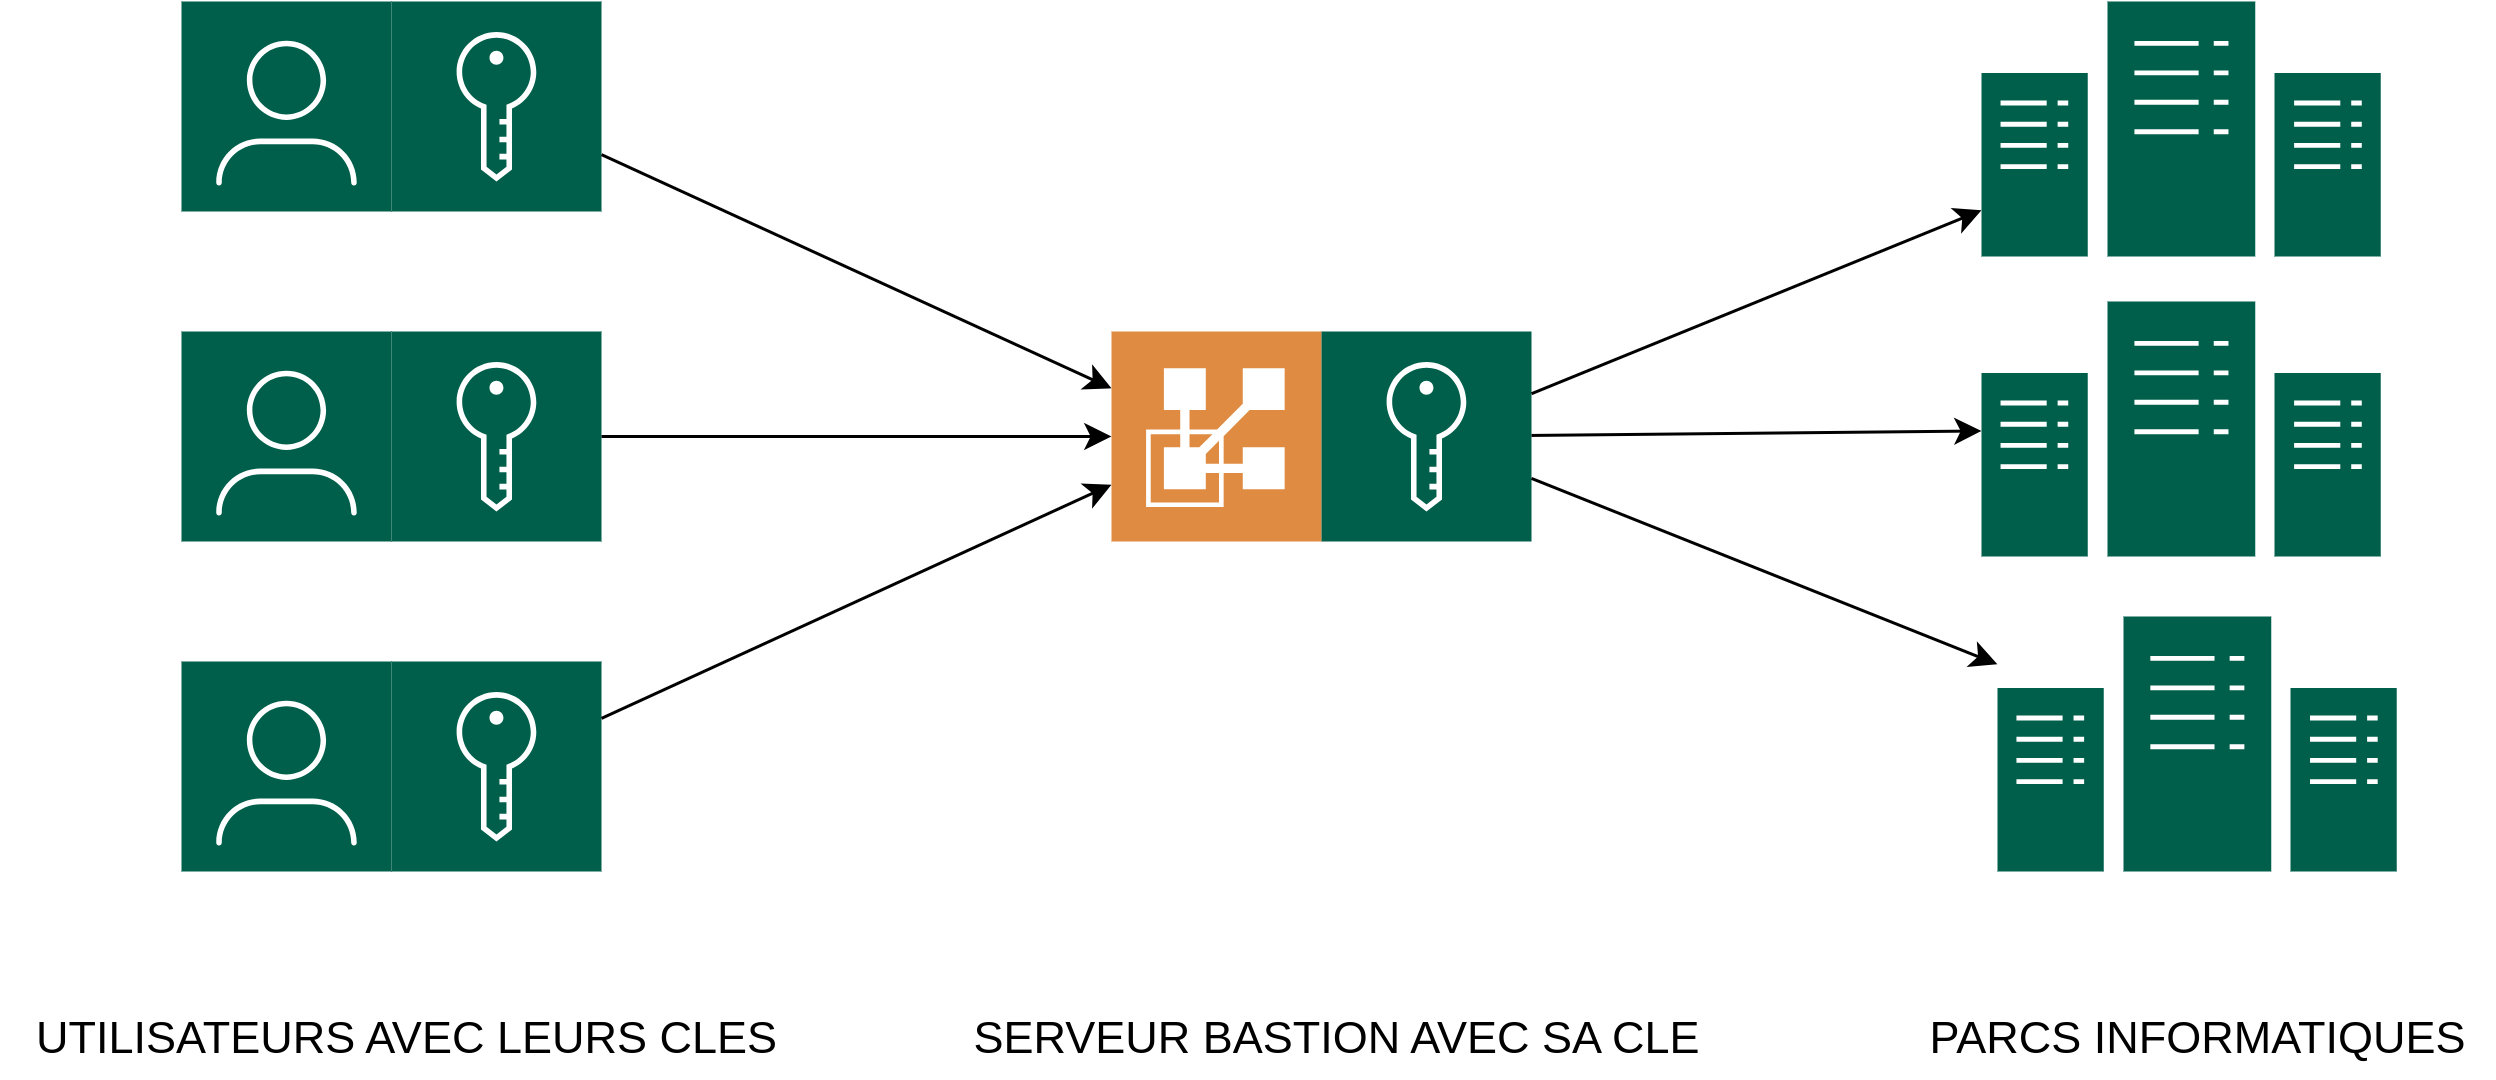
\includegraphics[scale = 0.15]{images/bastion.png}
  \caption{Utilisateurs accédant à distance à leurs parcs informatiques en se servant d'un serveur bastion.}  
  \label{fig:bastion} % pour la citer après
\end{figure}

J'ai donc commencé l'étude pour le choix d'une solution pour un serveur bastion, de son implémentation et de son maintient.
\\ \\
J'ai apprécié ce rapport à la sécurité dans cet exercice, en cours de complétion. Celui-ci permettra de renforcer la sécurité d'ADITU en ségmentarisant les accès aux machines aux personnes en ayant uniquement le besoin, et ce facilement. Répondant au problème initial que tout le monde avait accès à toutes les machines.

\subsubsection{Conceptualisation et intégration d'une nouvelle solution de supervision}

\underline{\textbf{je préfère attendre les premiers retours pour commencer à rédiger}}
\underline{\textbf{pour ne pas faire fausse route dès le départ et prendre du temps}}

\subsubsection{Réorganisation des réseaux privés virtuels des clients en data centres}

\underline{\textbf{je préfère attendre les premiers retours pour commencer à rédiger}}
\underline{\textbf{pour ne pas faire fausse route dès le départ et perdre du temps}}

\subsection{Activités annexes}

D'autres activités m'ont aussi permis de monter en compétences et de mieux m'accomoder au monde de l'entreprise : la prise de séances de formation.

\subsubsection{Suivi de séances de formation}

\textit{pourquoi j'avais besoin de formations + dire qu'au début je ne voyais pas pourquoi (j'ai appris : que je pouvais y assister pour aider les autres)}
\\
\textit{organisation des formations dans la semaine, dans quel but initial}
\\
\textit{ce que cela m'a apporté, pourquoi ça m'a aidé (explications, voir une vision différente d'une même notion)}

\subsubsection{Déplacements sur sites en clientèles et d'ADITU}

\textit{pourquoi j'ai eu besoin de me déplacer : la raison à chaque fois, pour apprendre}
\\ \\
\textit{déplacements sur site client pour de l'installation où j'ai aidé (soliha), et à dax pour apprendre et visualiser}
\\ \\
\textit{répondre à : est-ce que j'ai envie d'en refaire, est-ce que la clientèle m'intéresse}

\subsection{Bilan horaire et de compétences}

\textit{ici un diagramme de gantt de mes semaines pour montrer sur chacune des 29 semaines chez ADITU sur quoi j'étais (les services montés, puis sur iTop mais d'autres choses en parallèle...) pour leur donner le temps}
\\ \\
\textit{je mettrai aussi un diagramme camembert des domaines que j'ai touché, le quoi\\
réseaux 30\%
\\
développement et étude 25\%
\\
administration 20\%
\\
sécurité 10\%
\\
déplacements 10\%
\\
formations 5\%}

\newpage
\section{Conclusion et perspectives}
\label{conclusion}

Lors de cette année d'apprentissage, j'ai été amené à aborder des sujets d'études toujours plus complexes pour mes projets, pour la plupart en totale autonomie. Cette année m'a permis d'apprendre des compétences clés en entreprise que je n'aurai soupçonnées par des besoins personnels : comment monter efficacement une étude comparative et budgétaire, évoluer dans sa communication client et interne, découvrir le véritable besoin d'un client devant une demande etc.
\\ \\
%tout cela en supplément de ma montée en compétences sur tous les domaines techniques que j'ai abordés.
\\ \\
J'ai toujours essayé d'apprendre et d'évoluer dans mon travail plutôt que d'avancer le plus vite possible afin de rendre un projet rapidement. Pour ce faire, j'ai appris à documenter mon travail pour au mieux le conserver. J'en ai donc fait un suivi, mais aussi participé à des formations que je n'aurai pas besoin de faire deux fois. Pareil pour mes apprentissages d'outils : ayant écrit des procédures pour les actions les plus utiles et/ou complexes pour ces outils.
\\ \\
Je retiens que l'accomplissions d'un projet ne se termine pas lorsque nous avons fini ce qu'il nous était demandé de faire, mais quand le besoin initial relevant de celui-ci a été répondu. Ainsi, je me suis donné libre court de proposer de nouvelles directions dans mes projets, chose que je trouvais normale lorsque j'avais finalement cerné le besoin initial de ce projet et que je trouvais que la direction de son développement n'allait pas dans ce sens.


\section{Bilan personnel}

En dehors de ces compétences, cette année m'a aussi permis comportementalement d'évoluer sur mes principes d'explications et de raisonnement face à un besoin ou à un problème; initiés par le changement de la solution de support. Pareil du point de vue sécuritaire, je m'efforce désormais dans les services que je monte de trouver le juste milieu entre la sécurité et l'usage pratique pour les utilisateurs.
\\ \\
Être extrêmement bien encadré m'a aussi beaucoup aidé et je retiendrai l'importance d'être intégré dans une équipe. Il faut savoir développer son savoir être et savoir vivre avec ses collègues pour au mieux s'entendre avec eux, les comprendre et avancer efficacement. C'est sincèrement une valeur forte que j'ai apprise.
\\ \\
Je retiens aussi que je dois m'améliorer sur ma vision d'ensemble de mes projets - pas que professionnels -, résumé en une phrase : le mieux est l'ennemi du bien. Je dois réfléchir plusieurs fois avant de vouloir ajouter ou proposer quelque chose. De plus, vouloir toujours mieux faire conduira à ce que le projet n'aboutisse jamais. Mais encore, réinventer la roue sur chaque aspect ne sert à rien s'il n'y en a pas le besoin, car il y a pas besoin de faire mieux, juste de répondre à un objectif déterminé.

\newpage

\printbibliography % [title={Whole bibliography}

\newpage
\label{glossaire}

\setglossarystyle{listhypergroup}
\glsaddallunused
\printglossary[type=\acronymtype, title={Liste des abréviations}]
\printglossary[title={Glossaire}]

\newpage
\appendix

\section{Annexes}
\label{ddrs}
\subsection{fiche de poste}
\subsection{zone chalandise}
\subsection{itop}

\end{sloppypar}


\end{document}
